\chapter{Rencontre avec le C}

Maintenant que les présentations sont faites, il est temps de
découvrir les outils nécessaires pour programmer en C. Le strict
minimum pour programmer se résume en trois points :

\begin{itemize}

\item un \textbf{éditeur de texte} (à ne pas confondre avec un
  \textbf{traitement de texte} comme \emph{Microsoft Word} ou
  \emph{LibreOffice Writer}) : ce logiciel va servir à l'écriture du
  code source. Techniquement, n'importe quel éditeur de texte suffit,
  mais il est souvent plus agréable d'en choisir un qui n'est pas trop
  minimaliste ;
\item
  un \textbf{compilateur} : c'est le logiciel le plus important
  puisqu'il va nous permettre de transformer le code écrit en langage C
  en un fichier exécutable ;
\item un \textbf{débogueur} (ou \emph{debugger} en anglais) : ce
  logiciel vous sera très utile en cas de problèmes pour rechercher
  d'éventuelles erreurs dans votre programme.
\end{itemize}

À partir de là, il existe deux solutions : utiliser ces trois
logiciels séparément ou bien les utiliser au sein d'un
\textbf{environnement intégré de développement} (abrégé EDI). Dans le
cadre de ce cours, nous avons choisi la première option,
majoritairement dans un souci de transparence et de simplicité. En
effet, si les EDI peuvent être des compagnons de choix, ceux-ci sont
avant tout destinés à des programmeurs expérimentés et non à de
parfaits débutants

\section{Windows} 

\subsection{Le compilateur}

Nous vous proposons de télécharger MinGW, qui est une adaptation pour
Windows du compilateur GCC.

Rendez-vous sur le \MYhref{http://www.mingw.org/}{site de MinGW} dans
la section « \emph{download} » et cliquez sur le lien en haut de la
page « \emph{looking for the latest version ? Download
  mingw-get-install-xxxxxxxx.exe (xxx.x kB)} ».

Exécutez le programme, cliquez sur « \emph{install} », décochez la
case « \emph{also install support for graphical user interface} » et
enfin cliquez sur « \emph{continue} ».

Ceci étant fait, il nous faut désormais créer une variable
d'environnement afin de spécifier à notre invite de commande le chemin
vers les différents composants de MinGW.

\begin{itemize}
\item sous Windows XP et antérieur, faites un clic-droit sur « poste
  de travail » puis choisissez « propriétés ». Dans la fenêtre qui
  s'ouvre, cliquez sur « avancés » puis sur « variables
  d'environnement » ;
\item sous Windows Vista, Seven, faites un clic-droit sur l'icône «
  ordinateur » dans le menu « démarrer » ou bien sur « poste de
  travail ». Ensuite, cliquez sur « paramètres systèmes avancés
  ». Dans la nouvelle fenêtre qui s'ouvre, cliquez sur « variables
  d'environnement » ;
\item sous Windows 8, rendez-vous dans le panneau de configuration à
  la rubrique « système ». Cliquez sur « avancé » puis sur « variables
  d'environnement ».
\end{itemize}

\bigbreak

Dans la partie « utilisateur courant », créez une nouvelle variable
nommée \mybox{PATH} et donnez lui pour valeur :
\mybox{\%PATH\%;C:\textbackslash{}MinGW\textbackslash{}bin} (le chemin
après le point-virgule peut varier en fonction de où vous avez décidés
d'installer MinGW, l'important est de bien avoir le répertoire
\mybox{bin} à la fin).

À présent, exécutez l'invite de commandes (il est situé dans les
accessoires sous le même nom) et entrez la ligne suivante.

\begin{bash}
  mingw-get install gcc gdb
\end{bash}

Le compilateur et le débogueur sont à présent installés. À présent,
lancez le bloc-note et placez y le texte suivant.

\begin{bash}
  @echo off gcc -D__USE_MINGW_ANSI_STDIO=1 -Wall -Wextra -pedantic -std=c89 -fno-common
    -fno-builtin %*
\end{bash}

Ensuite, enregistrez ce fichier dans le dossier « bin » de MinGW (par
défaut \mybox{C:\textbackslash{}MinGW\textbackslash{}bin}) sous le nom
« zcc.bat » en choisissant « autres types de fichiers ».

Maintenant, rendez-vous dans le menu des accessoires, réalisez un clic
droit sur l'invite de commande et sélectionnez « propriétés ». Dans
l'onglet « raccourci », remplacer le champ « cible » par
«\%windir\%\textbackslash system32\textbackslash cmd.exe /k ``chcp
65001'' ». Enfin, dans l'onglet « police », choisissez « Consolas » ou
« Lucida Console » et adaptez la taille suivant vos envies.

\section{L'éditeur de texte}\label{luxe9diteur-de-texte-1}

L'éditeur de texte va nous permettre d'écrire notre code source et de
l'enregistrer. L'idéal est d'avoir un éditeur de texte facile à
utiliser et pas trop minimaliste. Si jamais vous avez déjà un éditeur
de texte et que vous l'appréciez, n'en changez pas, il fera sûrement
l'affaire.

Si vous n'avez pas d'idée, nous vous conseillons
\MYhref{http://notepad-plus-plus.org/fr/}{Notepad++} qui est simple,
pratique et efficace. Pour le télécharger, rendez-vous simplement dans
la rubrique « Téléchargements » du menu principal.

\begin{infobox}
 Veillez-bien à ce que l'encodage de
votre fichier soit « UTF-8 (sans BOM) » (voyez le menu éponyme à cet
effet).
\end{infobox}

\section{Introduction à la ligne de
  commande}\label{introduction-uxe0-la-ligne-de-commande-1}

La ligne de commande, derrière son aspect rustre et archaïque, n'est
en fait qu'une autre manière de réaliser des tâches sur un
ordinateur. La différence majeure avec une interface graphique étant
que les instructions sont données non pas à l'aide de boutons et de
cliques de souris, mais exclusivement à l'aide de texte. Ainsi, pour
réaliser une tâche donnée, il sera nécessaire d'invoquer un programme
(on parle souvent de \textbf{commandes}) en tapant son nom.

La première chose que vous devez garder à l'esprit, c'est le dossier
dans lequel vous vous situez. Celui-ci est indiqué au tout début de
chaque ligne et se termine par le symbole \mybox{\textgreater{}}. Ce
dossier est celui dans lequel les actions (par exemple la création
d'un répertoire) que vous demanderez seront réalisées. Normalement,
par défaut, vous devriez vous situez dans le répertoire
\mybox{C:\textbackslash{}Users\textbackslash{}Utilisateur} (où
\mybox{Utilisateur} correspond à votre nom d'utilisateur). Ceci étant
posé, voyons quelques commandes basiques.

La commande \mybox{mkdir} (pour \emph{make directory}) vous permet de
créer un nouveau dossier. Pour ce faire, tapez \mybox{mkdir} suivi
d'un espace et du nom du nouveau répertoire. Par exemple, vous pouvez
créer un dossier « Programmation » comme suit.

\begin{bash}
  C:\Users\Utilisateur> mkdir Programmation
\end{bash}

La commande \mybox{dir} (pour \emph{directory}) vous permet de lister
le contenu d'un dossier. Vous pouvez ainsi vérifier qu'un nouveau
répertoire a bien été créé.

\begin{bash}
  C:\Users\Utilisateur> dir Répertoire de C:\Users\Utilisateur

  30/03/2015 17:00 <REP> .  30/03/2015 17:00 <REP> ..  30/03/2015
  17:00 <REP> Programmation
\end{bash}

\begin{infobox}
  Le résultat ne sera pas forcément le même que ci-dessus, cela dépend
  du contenu de votre dossier. L'essentiel est que vous retrouviez
  bien le dossier que vous venez de créer.
\end{infobox}

Enfin, la commande \mybox{cd} (pour \emph{change directory}) vous
permet de vous déplacer d'un dossier à l'autre. Pour ce faire,
spécifiez simplement le nom du dossier de destination.

\begin{bash}
  C:\Users\Utilisateur> cd Programmation
  C:\Users\Utilisateur\Programmation>
\end{bash}

\begin{infobox}
Le dossier spécial « \textbf{..} »
représente le répertoire parent. Il vous permet donc de revenir en
arrière dans la hiérarchie des dossiers. Le dossier spécial «
\textbf{.}  » représente quant à lui le dossier courant.
\end{infobox}

Voilà, avec ceci, vous êtes fin prêt pour compiler votre premier
programme. Vous pouvez vous rendre à la deuxième partie de ce
chapitre.

\emph{{[}MinGW{]}: Minimalist GNU for Windows }{[}GCC{]}: GNU Compiler
Collection.

\section{GNU/Linux, *BSD et autres Unixoïdes}

\subsection{ Le compilateur}\label{le-compilateur}

Suivant le système que vous choisissez, vous aurez ou non le choix
entre différents compilateurs. Si vous n'avez pas d'idée, nous vous
conseillons d'opter pour GCC en installant le paquet éponyme à l'aide
de votre gestionnaire de paquet. Également, vous pouvez installer le
paquet « gdb » qui est un débogueur.

\subsection{Configuration}\label{configuration-1}

Ceci dépend de votre interpréteur de commande. Pour savoir quel est
celui dont vous disposez, ouvrez un terminal (le plus souvent, vous
pouvez y accéder via la catégorie « accessoires » de votre menu
principal) et entrez la commande suivante.

\begin{bash}
  echo $SHELL
\end{bash}


\subsubsection{bash}\label{bash}

Exécutez la commande suivante depuis votre dossier personnel (vous y
êtes par défaut au lancement de l'invite de commande).

\begin{bash}
  echo "alias zcc='gcc -Wall -Wextra -pedantic -std=c89 -fno-common -fno-builtin'"
  >> .bashrc
\end{bash}


\subsubsection{csh ou tcsh}\label{csh-ou-tcsh}

Exécutez la commande suivante depuis votre dossier personnel (vous y
êtes par défaut au lancement de l'invite de commande).

\begin{bash}
  echo "alias zcc 'gcc -Wall -Wextra -pedantic -std=c89 -fno-common -fno-builtin'"
  >> .cshrc # (ou .tcshrc)
\end{bash}


\subsubsection{ksh, zsh ou sh}\label{ksh-zsh-ou-sh}

Exécutez les commandes suivante depuis votre dossier personnel (vous y
êtes par défaut au lancement de l'invite de commande).

\begin{bash}
  echo "alias zcc='gcc -Wall -Wextra -pedantic -std=c89 -fno-common -fno-builtin'"
  >> .kshrc # (ou .zshrc ou .shrc) echo "export ENV=\$HOME.kshrc"
  >> .profile # (ou .zshrc ou .shrc)
\end{bash}

\subsection{L'éditeur de texte}\label{luxe9diteur-de-texte-2}

Ce serait un euphémisme de dire que vous avez l'embarras du choix. Il
existe une pléthore d'éditeurs de texte fonctionnant en ligne de
commande ou avec une interface graphique, voire les deux.

Pour n'en citer que quelques-uns, en ligne de commande vous trouverez
par exemple : Vim et Emacs (les deux monstres de l'édition), Nano ou
Joe. Côté graphique, vous avez entre autres : Gedit, Mousepad et Kate.

\subsection{Introduction à la ligne de
  commande}\label{introduction-uxe0-la-ligne-de-commande-2}

La ligne de commande, derrière son aspect rustre et archaïque, n'est
en fait qu'une autre manière de réaliser des tâches sur un
ordinateur. La différence majeure avec une interface graphique étant
que les instructions sont données non pas à l'aide de boutons et de
cliques de souris, mais exclusivement à l'aide de texte. Ainsi, pour
réaliser une tâche donnée, il sera nécessaire d'invoquer un programme
(on parle souvent de \textbf{commandes}) en tapant son nom.

La première chose que vous devez garder à l'esprit, c'est le dossier
dans lequel vous vous situez. Suivant le terminal que vous employez,
celui-ci est parfois indiqué en début de ligne et terminé par le
symbole \mybox{\$} ou \mybox{\%}. Ce dossier est celui dans lequel les
actions (par exemple la création d'un répertoire) que vous demanderez
seront exécutées. Normalement, par défaut, vous devriez vous situez
dans le répertoire : \mybox{/home/utilisateur} (où \mybox{utilisateur}
correspond à votre nom d'utilisateur). Ceci étant posé, voyons
quelques commandes basiques.

La commande \mybox{pwd} (pour \emph{print working directory}) vous
permet de connaître le répertoire dans lequel vous êtes.

\begin{bash}
  $ pwd /home/utilisateur
\end{bash}

La commande \mybox{mkdir} (pour \emph{make directory}) vous permet de
créer un nouveau dossier. Pour ce faire, tapez \mybox{mkdir} suivi
d'un espace et du nom du nouveau répertoire. Par exemple, vous pouvez
créer un dossier « programmation » comme suit :

\begin{bash}
  $ mkdir programmation
\end{bash}

La commande \mybox{ls} (pour \emph{list}) vous permet de lister le
contenu d'un dossier. Vous pouvez ainsi vérifier qu'un nouveau
répertoire a bien été créé.

\begin{bash}
  $ ls programmation
\end{bash}

\begin{infobox}
  Le résultat ne sera pas forcément le même que ci-dessus, cela dépend
  du contenu de votre dossier. L'essentiel est que vous retrouviez
  bien le dossier que vous venez de créer.
\end{infobox}

Enfin, la commande \mybox{cd} (pour \emph{change directory}) vous
permet de vous déplacer d'un dossier à l'autre. Pour ce faire,
spécifiez simplement le nom du dossier de destination.

\begin{bash}
  $ cd programmation 
  $ pwd /home/utilisateur/programmation
\end{bash}

\begin{infobox}
Le dossier spécial « \textbf{..} »
représente le répertoire parent. Il vous permet donc de revenir en
arrière dans la hiérarchie des dossiers. Le dossier spécial «
\textbf{.}  » représente quant à lui le dossier courant.
\end{infobox}

Voilà, avec ceci, vous êtes fin prêt pour compiler votre premier
programme. Vous pouvez vous rendre à la deuxième partie de ce
chapitre.

*{[}GCC{]}: GNU Compiler Collection

\section{Mac OS X}

\subsection{Le compilateur}

Allez dans le dossier \mybox{/Applications/Utilitaires} et lancez
l'application « terminal.app ». Une fois ceci fait, entrez la commande
suivante :

\begin{bash}
xcode-select --install
\end{bash}

et cliquez sur « installer » dans la fenêtre qui apparaît. Si vous
rencontrez le message d'erreur ci-dessous, cela signifie que vous
disposez déjà des logiciels requis.

\begin{bash}
  Impossible d’installer ce logiciel car il n’est pas disponible
  actuellement depuis le serveur de mise à jour de logiciels.
\end{bash}

Si vous ne disposez pas de la commande indiquée, alors rendez-vous sur
le site de développeur d'Apple :
\MYhref{https://developer.apple.com/}{\emph{Apple developer
    connection}}.  Il faudra ensuite vous rendre sur le « \emph{mac
  dev center} » puis, dans « \emph{additional download} », cliquez sur
« \emph{view all downloads} ». Quand vous aurez la liste, il vous
suffit de chercher la version 3 de Xcode (pour Leopard et Snow
Leopard) ou 2 pour les versions antérieures (Tiger). Vous pouvez aussi
utiliser votre CD d'installation pour installer Xcode (sauf pour
Lion).

\subsection{Configuration}\label{configuration}

Voyez ce qui est dit pour GNU/Linux, *BSD et les autres Unixoïdes.

\subsection{L'éditeur de texte}\label{luxe9diteur-de-texte}

Comme pour les autres Unixoïdes, vous trouverez un bon nombres
d'éditeurs de texte. Si toutefois vous êtes perdu, nous vous
conseillons
\MYhref{http://www.barebones.com/products/TextWrangler/}{TextWrangler}
ou \MYhref{https://www.peterborgapps.com/smultron/}{Smultron}.

\subsection{Introduction à la ligne de
commande}\label{introduction-uxe0-la-ligne-de-commande}

Référez-vous à l'introduction dédiée à GNU/Linux, *BSD et les autres
Unixoïdes.

\section{Notre cible}

Avant de commencer à programmer, il nous faut aussi définir ce que
nous allons programmer, autrement dit le type de programme que nous
allons réaliser. Il existe en effet deux grands types de programmes :
les programmes \textbf{graphiques} et les programmes \textbf{en
  console}.

Les programmes graphiques sont les plus courants et les plus connus
puisqu'il n'y a pratiquement qu'eux sous Windows ou Mac OS X par
exemple. Vous en connaissez sans doute énormément tel que les lecteurs
de musique, les navigateurs Internet, les logiciels de discussions
instantanées, les suites bureautiques, les jeux vidéos, etc. Ce sont
tous des programmes graphiques, ou programmes GUI. En voici un exemple
sous GNU/Linux.

\begin{figure}[!ht]
\centering
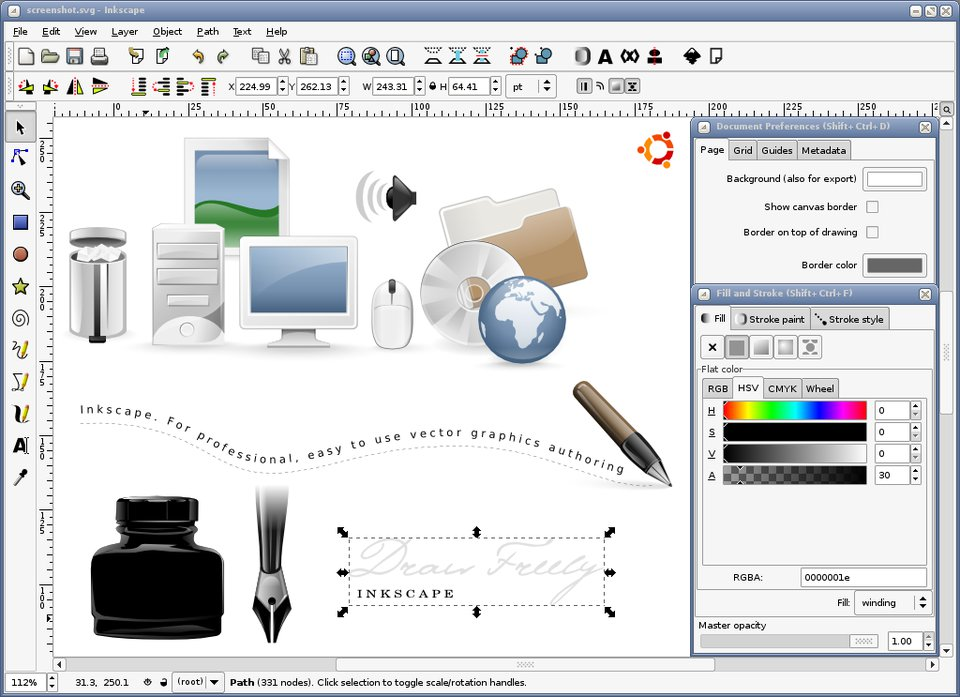
\includegraphics[scale=0.4]{images/Inskape_screenshot.jpg}
\caption{L'éditeur d'images vectorielles Inkscape est un programme
graphique}
\end{figure}

Cependant, écrire ce genre de programmes demande beaucoup de
connaissances, ce qui nous manque justement pour l'instant. Aussi,
nous allons devoir nous rabattre sur le deuxième type de programme :
les programmes en console.

Les programmes console sont les premiers programmes et sont apparus en
même temps que l'écran. Ils étaient très utilisés dans les années
1970/1980 (certains d'entre vous se souviennent peut-être de MS-DOS),
mais ont fini par être remplacés par une interface graphique avec la
sortie de Mac OS et de Windows. Cependant, ils existent toujours et
redeviennent quelque peu populaires chez les personnes utilisant
GNU/Linux ou un *BSD.

Voici un exemple de programme en console (il s'agit de
\MYhref{http://www.gnu.org/software/chess/}{GNU Chess}, un jeu
d'échecs performant entièrement en ligne de commande).

\begin{bash}
White (1) : d4
1. d4

black  KQkq  d3
r n b q k b n r 
p p p p p p p p 
. . . . . . . . 
. . . . . . . . 
. . . P . . . . 
. . . . . . . . 
P P P . P P P P 
R N B Q K B N R 

Thinking...

white  KQkq
r n b q k b . r 
p p p p p p p p 
. . . . . n . . 
. . . . . . . . 
. . . P . . . . 
. . . . . . . . 
P P P . P P P P 
R N B Q K B N R 


My move is : Nf6
White (2) :
\end{bash}

Ce sera le type de programme que nous allons apprendre à créer.
Rassurez-vous, quand vous aurez fini le cours, vous aurez les bases
pour apprendre à créer des programmes graphiques. Tout est possible.

\section{Première rencontre}

Bien, il est à présent temps d'écrire et de compiler notre premier
programme ! Pour ce faire, ouvrez votre éditeur de texte et entrez les
lignes suivantes.

\begin{C}
  int main(void)
  {
    return 0
  }
\end{C}

Ensuite, enregistrez ce fichier dans un dossier de votre choix et
nommez-le « main.c ». Une fois ceci fait, rendez-vous dans le dossier
contenant le fichier à l'aide d'un terminal et exécutez la commande
ci-dessous.

\begin{C}
zcc main.c
\end{C}

\clearpage

\begin{attentionbox}
  Si vous n'êtes pas sous Windows et que vous utilisez
  l'interprétateur de commande \mybox{sh}, \mybox{ksh} ou \mybox{zsh},
  la commande \mybox{zcc} ne sera connue de votre invite de commande
  qu'une fois que vous aurez ouvert une nouvelle session. En
  attendant, vous pouvez entrez la commande \mybox{alias zcc='gcc
    -Wall -Wextra -pedantic -std=c89 -fno-common -fno-builtin'} dans
  votre terminal pour que cela fonctionne.
\end{attentionbox}

Si tout se passe bien, vous devriez obtenir un fichier « a.exe » sous
Windows et un fichier « a.out » sinon. Vous pouvez exécutez ce programme
en tapant \mybox{a.exe} ou \mybox{./a.out}.

\begin{questionbox}
  Je viens de le faire, mais il ne se passe rien
\end{questionbox}


Cela tombe bien, c'est exactement ce que fait ce programme : rien. :p
Voyons cela plus en détails.

Ce bout de code est appelé une \textbf{fonction}. Un programme écrit en
C n'est composé pratiquement que de fonctions qui sont des morceaux de
programme donnant des instructions à l'ordinateur. Elles ont toujours un
objectif, une \emph{fonction} particulière, par exemple calculer la
racine carrée d'un nombre.

Notre fonction s'appelle \mybox{main} (prononcez « mèïne »). C'est la
fonction de base commune à tous les programmes en C, le programme
commence et finit toujours par elle.

Une fonction est délimitée par des accolades (\mybox{\{} et
\mybox{\}}). Après les accolades, il n'y a rien, car pour l'instant
nous n'avons que la fonction \mybox{main}.

Le nom de la fonction est précédé du mot-clé \mybox{int} qui est un nom
de type (nous verrons cette notion au chapitre suivant) qui indique que
la fonction retourne une valeur entière. À l'intérieur des parenthèses,
il y a le mot \mybox{void} qui signifie que la fonction ne reçoit pas
de paramètres, nous y reviendrons en temps voulu.

Enfin, la fonction se termine par l'instruction \mybox{return 0} qui
signifie en l'occurrence que la fonction a terminé son travail (bon,
pour l'instant elle n'en a pas, mais nous y arriverons rapidement) et
que tout s'est bien passé.

\section{Les commentaires}

Il est souvent nécessaire de \textbf{commenter son code source} pour
décrire des passages un peu moins lisibles ou tout simplement pour
offrir quelques compléments d'information au lecteur du code. Nous en
utiliserons souvent dans la suite de ce cours pour rendre certains
exemples plus parlant.

Un commentaire est ignoré par le compilateur, il disparait et n'est
pas présent dans l'exécutable. Il ne sert qu'au programmeur et aux
lecteurs du code.

Un commentaire en C est écrit entre les signes \mybox{/*} et
\mybox{*/} et peut très bien prendre plusieurs lignes.

\begin{C}
/* Ceci est un commentaire. */
\end{C}


\begin{C}
/* Ceci est un commentaire qui

prend plusieurs lignes. */
\end{C}

Voilà, vous avez enfin fait la connaissance du C à travers du
code. Certes, nous n'avons vu qu'un petit code et avons seulement
survolé les différents éléments, mais il n'empêche que cela représente
certainement beaucoup de nouveautés pour vous. Relisez donc ce
chapitre à tête reposée si nécessaire.
